\subsection{Architecture}
\label{sec:tool}
\begin{figure}[t!]
\centering
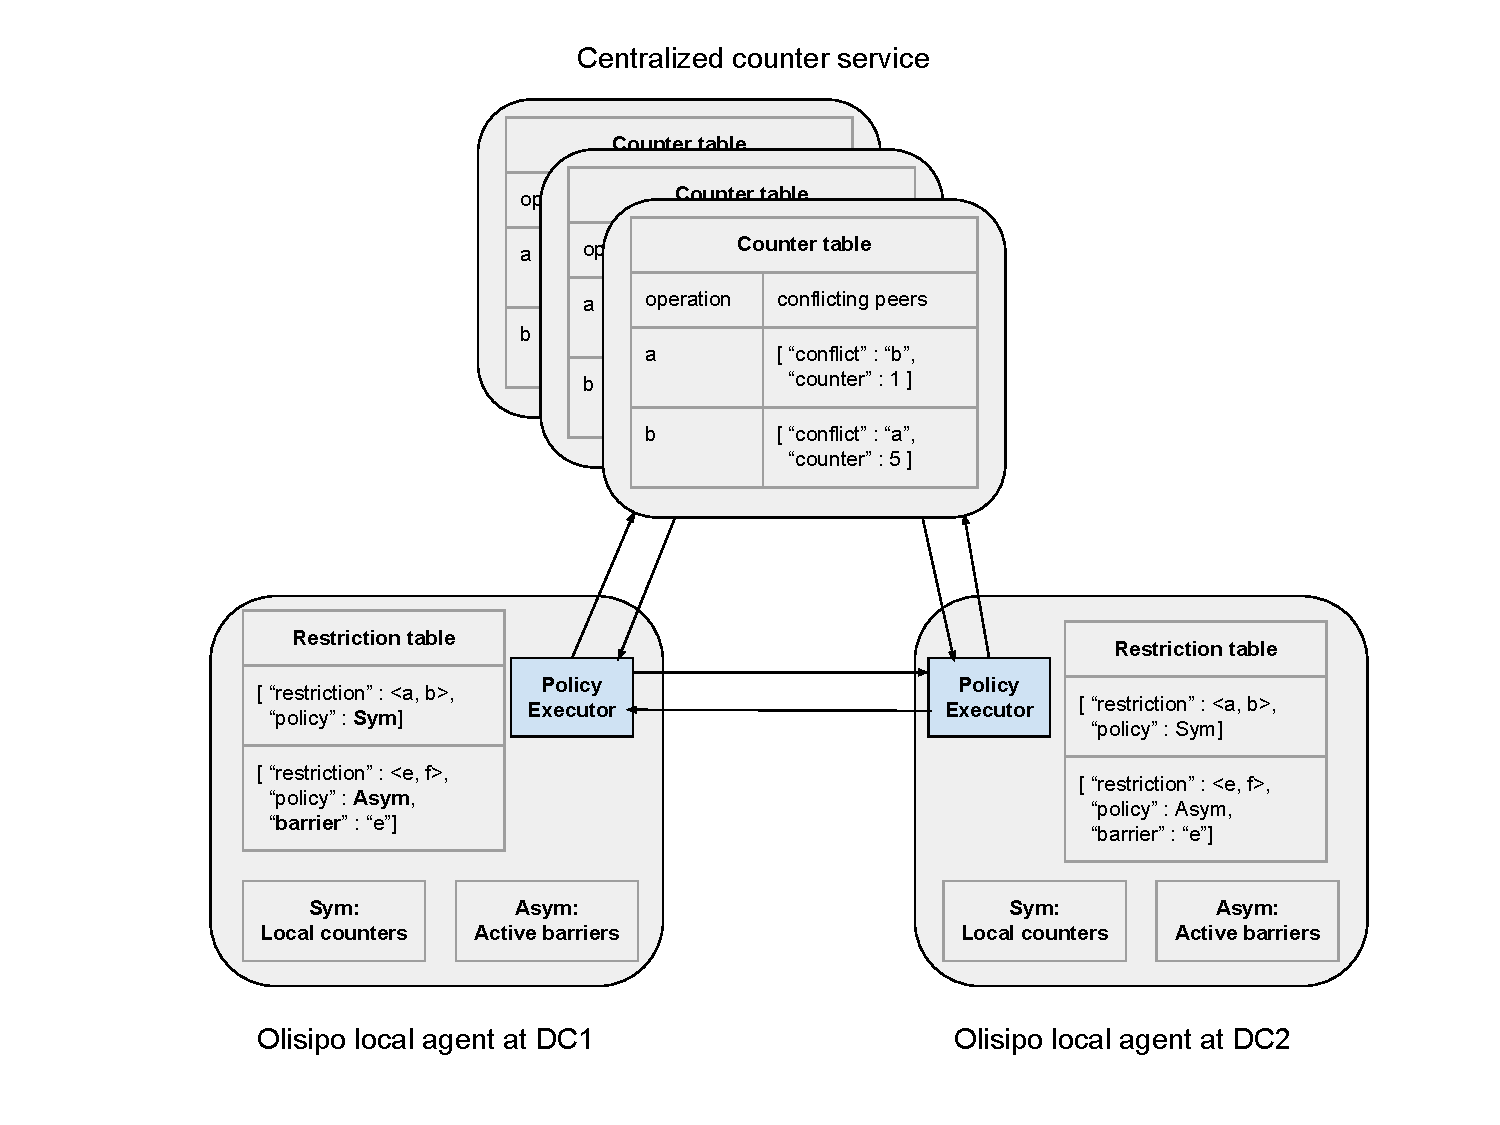
\includegraphics[width=\columnwidth]{./figures/tool_support.pdf}
\caption{\coordtool\ architecture}
\label{fig:tooldesign}
\end{figure}

All design choices and details presented above lead to the high level system architecture 
depicted in Figure~\ref{fig:tooldesign}. The \coordtool\ architecture consists of a replicated counter service across data centers and a local agent deployed
in every data center. While the counter service is required by executing the {\tt Sym} protocol
for keeping track of the number of different operations that have been accepted by the system.
the local agent is responsible for placing coordination only when the corresponding
operation is confined by restrictions. Every local agent keeps a restriction table, which defines
all identified restrictions between pair of operations and the corresponding coordination policy.
In addition, every agent also stores some meta data required for different protocols. With regard
to the {\tt Sym} protocol, it maintains a local copy of the replicated counter service, which is used
for learning if the local counters lag behind the global counters, which means
the corresponding data centers have to wait until all missing operations have been locally
incorporated. For the {\tt Asym} protocol, every agent maintains a list of active barriers, which
are used for locally deciding if the counterpart operations of such barriers can proceed or must wait.

\begin{figure}[t!]
\centering
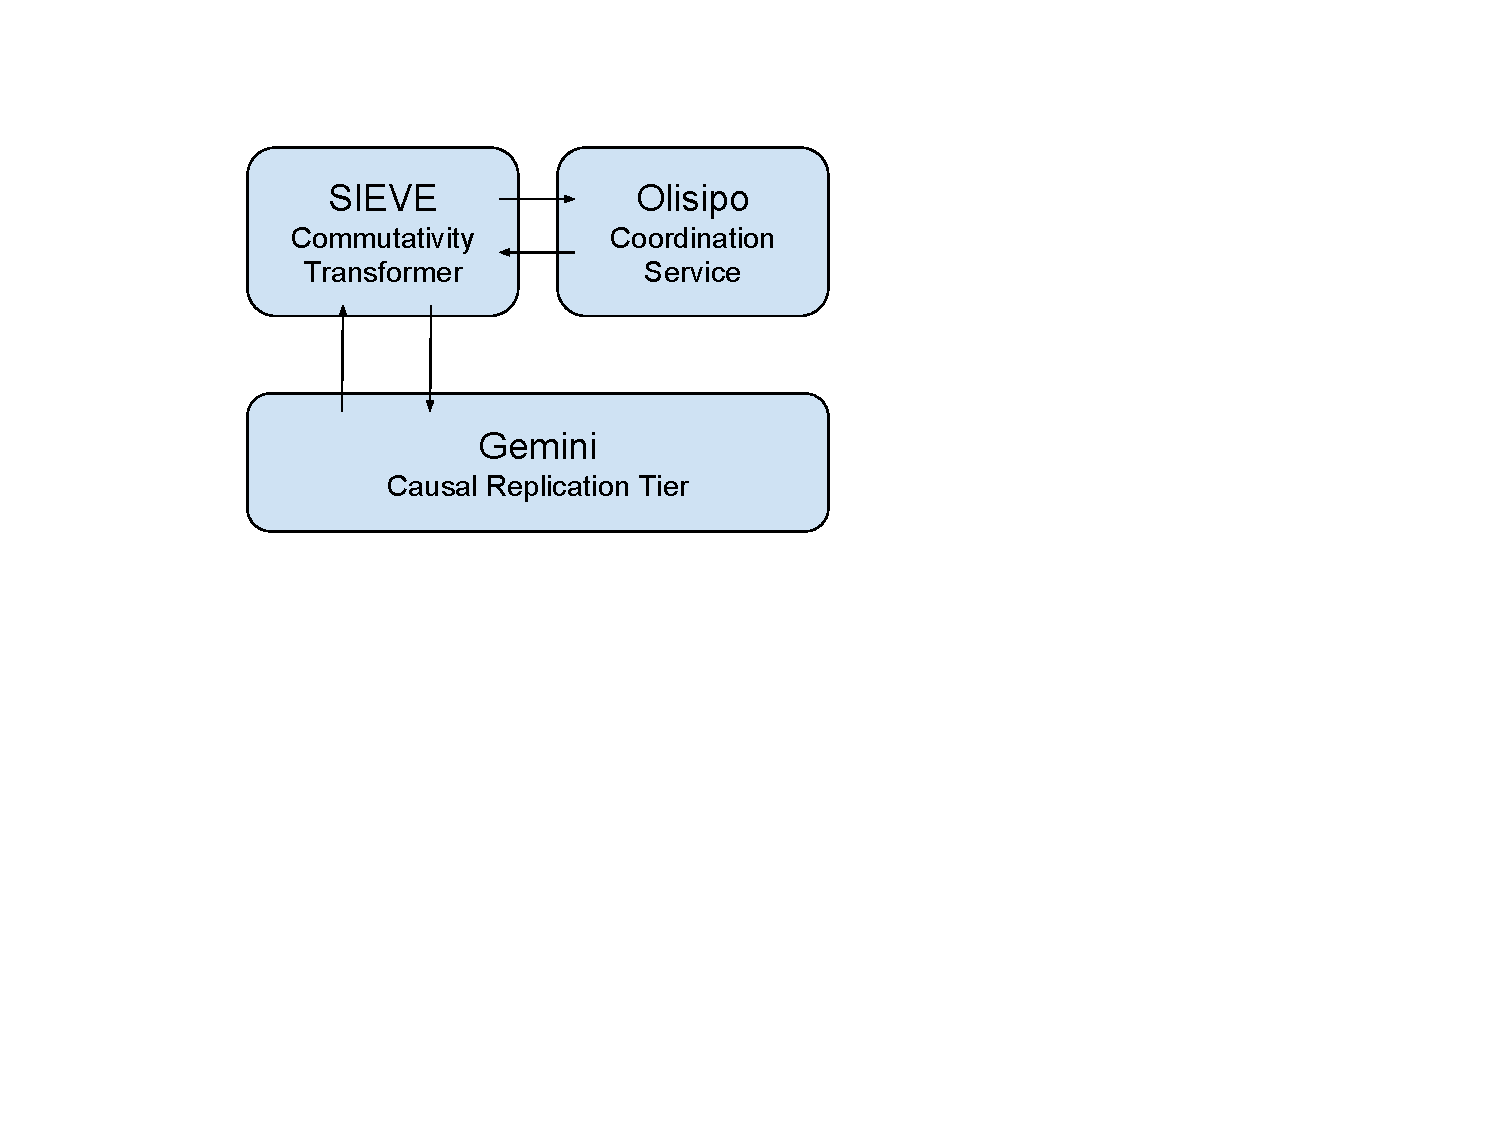
\includegraphics[width=0.76\columnwidth]{./figures/tool_intergated.pdf}
\caption{\coordtool\ connected with \tool\ and \gemini}
\label{fig:toolwithenvironment}
\end{figure}

\subsection{Implementation}
We implemented \coordtool\ using Java ($2.8k$ lines of code)~\footnote{The lines of code is
measured by {\tt cloc}~\cite{codecounter}.}, and used BFTSmart~\cite{bftsmartcode} for replicating
the state of the centralized counter service, MySQL as the backend storage, and Netty
as the communication library~\cite{Netty}. As shown in Figure~\ref{fig:toolwithenvironment},
we integrated \coordtool\ with \gemini\ and \tool\ so
that \gemini\ serves as the underlying causally consistent replication tier while \tool\ is used to
produce commutative shadow operations at runtime. 

\noindent\paragraph{Workflow:} A user issues her request to an application server locating at a nearby
data center, which runs a \tool\ library introduced in Chapter~\ref{chapter:sieve} and
a local agent shown in Figure~\ref{fig:tooldesign}. \tool\ intercepts the communication between
the app server and the backend MySQL database and executes the corresponding generator operation.
When the execution ends, \tool\ produces a commutative shadow operation that accumulates side effects
of that request, and then asks the \coordtool\ local agent for placing coordination if needed before committing and replicating
that shadow operation. To do so, \coordtool\ agent lookups into the restriction table
if that operation is confined by any restriction. If so, then the {\tt policy executor} residing
\coordtool\ orders that operation with respect to all its conflicting operations that are running concurrently
at other data centers. This is achieved by invoking a sequence of functions 
presented in Figure~\ref{fig:por:olisipinterface} associated with different protocols 
according to the lookup result, i.e., which protocols to be used. 
At the end, when conflicting operations are accordingly serialized, \tool\ sends these
operations to \gemini\ for replicating them across all data centers while respecting the established order. 
The sourcecode of \coordtool\ is available at ~\cite{olisipocode}.
